\documentclass[10pt,a4paper]{article}
\usepackage[utf8]{inputenc}

% Math environments and macros
\usepackage{amsmath}
\usepackage{amsfonts}
\usepackage{amssymb}
\usepackage{amsthm}

\usepackage{tikz}
\usetikzlibrary{automata}

% Define the page margin
\usepackage[margin=3cm]{geometry}

% Define \includegraphics to include graphics
\usepackage{graphicx}

% Better typography (font rendering)
\usepackage{microtype}

% Syntax highlighting
\usepackage{minted}

% Set global minted options
\setminted{linenos, autogobble, frame=lines, framesep=2mm}

\title{Distributed Systems, Sheet 1}
\author{Marten Lienen (03670270)}

\begin{document}

\maketitle

\section*{Exercise 1}

\subsection*{Server}

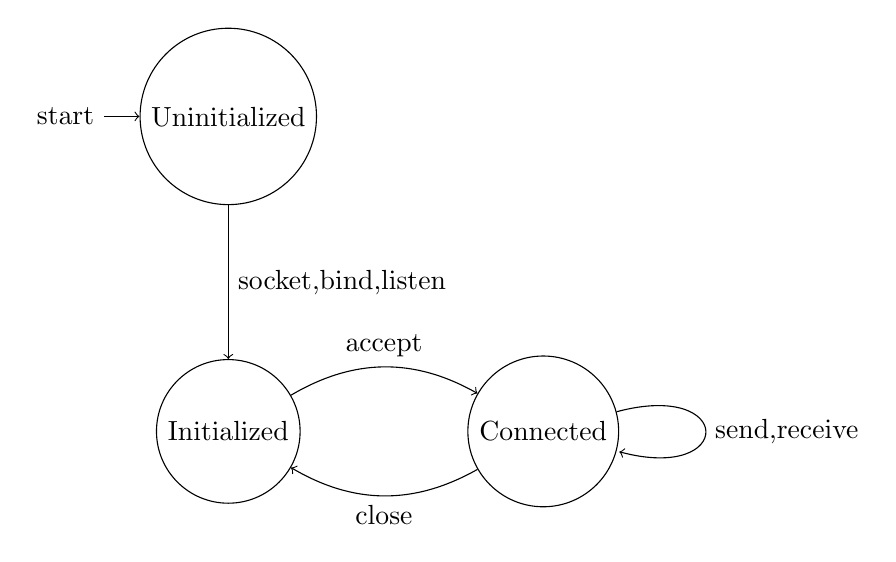
\begin{tikzpicture}[auto,node distance=4cm]
  \node[state,initial](uninit){Uninitialized};
  \node[state,below of= uninit](init){Initialized};
  \node[state,right of= init](connected){Connected};

  \path[->]
  (uninit) edge node {socket,bind,listen} (init)
  (init) edge [bend left] node {accept} (connected)
  (connected) edge [loop right] node {send,receive} (connected)
  (connected) edge [bend left] node {close} (init);
\end{tikzpicture}

\subsection*{Client}

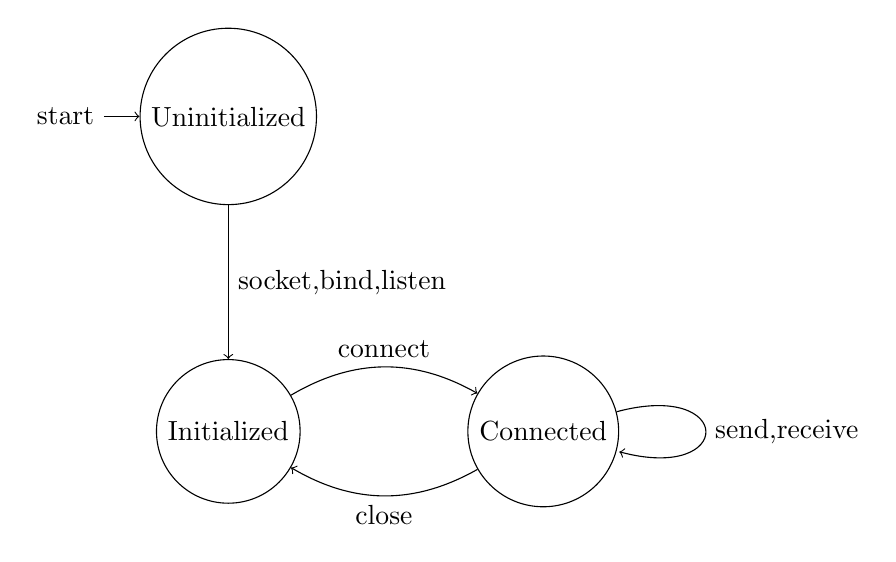
\begin{tikzpicture}[auto,node distance=4cm]
  \node[state,initial](uninit){Uninitialized};
  \node[state,below of= uninit](init){Initialized};
  \node[state,right of= init](connected){Connected};

  \path[->]
  (uninit) edge node {socket,bind,listen} (init)
  (init) edge [bend left] node {connect} (connected)
  (connected) edge [loop right] node {send,receive} (connected)
  (connected) edge [bend left] node {close} (init);
\end{tikzpicture}

\section*{Exercise 2}

\subsection*{Part a)}

\begin{minted}{ebnf}
  sign = "+" | "-" ;
  digit = "0" | "1" | "2" | "3" | "4" | "5" | "6" | "7" | "8" | "9" ;
  float = [ sign ], { digit }, ".", { digit } ;
  complex = float, "i", float ;
\end{minted}

\subsection*{Part b)}

\begin{minted}{ebnf}
  operator = "+", "*", "/", "-" ;
  m1 = complex, ",", complex, ",", operator, ";" ;
\end{minted}

\begin{minted}{python}
  ".32i5.,-1.i.,+;"
\end{minted}

\subsection*{Part c)}

\begin{minted}{ebnf}
  message = "SUCCESS", "DIVISION-BY-ZERO", "INVALID-INPUT" ;
  m2 = message, ",", complex, ";" ;
\end{minted}

\subsection*{Part d)}

Redefine the following parts
\begin{minted}{ebnf}
  operator = "+", "*", "/", "-", "polar" ;
  rectangular = float, "i", float ;
  polar = float, "r", float ;
  complex = rectangular | polar ;
\end{minted}

\subsection*{Part e)}

\subsubsection*{Successful}

\begin{minted}{python}
  -> 4.2i1.,-.8i2,-;
  <- SUCCESS,5.i3.;
\end{minted}

\subsubsection*{Erroneous}

\begin{minted}{python}
  -> YOLO%
  <- INVALID-INPUT,.i.;
\end{minted}

\subsection*{Part f)}

\begin{minted}{python}
  -> 3.i4.,1.i2.,+;
  <- SUCCESS,4.i6.;
\end{minted}

\section*{Exercise 3}

\subsection*{Part a)}

\subsubsection*{Client}

\begin{minted}{java}
  public String doRPC(String command, String ip, int port) {
    Socket sock = new Socket();
    sock.connect(ip, port);
    sock.send(command);

    return sock.receive();
  }
\end{minted}

\subsubsection*{Server}

\begin{minted}{java}
  public void provideService(int port) {
    ServerSocket ss = new ServerSocket(port);

    while (true) {
      Socket sock = ss.accept();
      sock.receive();
      sock.send("Result");
    }
  }
\end{minted}

\subsection*{Part b)}

\begin{minted}{java}
  class Complex {
    private double real;
    private double imaginary;

    public Complex(double real, double imaginary) {
      this.real = real;
      this.imaginary = imaginary;
    }

    public String marshal() {
      return "" + this.real + "i" + this.imaginary;
    }

    public static Complex unmarshal(String data) {
      String[] parts = data.split("i");

      return new Complex(parts[0].parseDouble(), parts[1].parseDouble());
    }
  }
\end{minted}

\subsection*{Part c)}

\subsection*{Part d)}

\subsection*{Part e)}

\begin{itemize}
\item They take up extra space
\item Alternatively define a schema with elements of known length, that can be pattern matched
\end{itemize}

\section*{Exercise 4}

\begin{itemize}
\item It is harder to program
\item Does not block a whole thread
\end{itemize}

\section*{Exercise 5}

\begin{minted}{java}
  selector = new Selector();

  ssc.bind("...", 1337);
  ssc.configureBlocking(false);
  ssc.register(selector, SelectionKey.ACCEPT);

  while (true) {
    selector.select();

    for (SelectionKey key : selector.selectedKeys()) {
      if (key.isAcceptable()) {
        SocketChannel sc = key.getChannel().accept();
        sc.configureBlocking(false);
        sc.register(selector, SelectionKey.READ | SelectionKey.WRITE);
      } else if (key.isWriteable()) {
        ((SocketChannel)key.getChannel()).write("Hello!");
      } else if (key.isReadable()) {
        // ...
      }
    }
  }
\end{minted}

\end{document}
